\PassOptionsToPackage{unicode=true}{hyperref} % options for packages loaded elsewhere
\PassOptionsToPackage{hyphens}{url}
%
\documentclass[english,,man]{apa6}
\usepackage{lmodern}
\usepackage{amssymb,amsmath}
\usepackage{ifxetex,ifluatex}
\usepackage{fixltx2e} % provides \textsubscript
\ifnum 0\ifxetex 1\fi\ifluatex 1\fi=0 % if pdftex
  \usepackage[T1]{fontenc}
  \usepackage[utf8]{inputenc}
  \usepackage{textcomp} % provides euro and other symbols
\else % if luatex or xelatex
  \usepackage{unicode-math}
  \defaultfontfeatures{Ligatures=TeX,Scale=MatchLowercase}
\fi
% use upquote if available, for straight quotes in verbatim environments
\IfFileExists{upquote.sty}{\usepackage{upquote}}{}
% use microtype if available
\IfFileExists{microtype.sty}{%
\usepackage[]{microtype}
\UseMicrotypeSet[protrusion]{basicmath} % disable protrusion for tt fonts
}{}
\IfFileExists{parskip.sty}{%
\usepackage{parskip}
}{% else
\setlength{\parindent}{0pt}
\setlength{\parskip}{6pt plus 2pt minus 1pt}
}
\usepackage{hyperref}
\hypersetup{
            pdftitle={Describing vocalizations in young children: A big data approach through citizen science annotation},
            pdfborder={0 0 0},
            breaklinks=true}
\urlstyle{same}  % don't use monospace font for urls
\usepackage{graphicx,grffile}
\makeatletter
\def\maxwidth{\ifdim\Gin@nat@width>\linewidth\linewidth\else\Gin@nat@width\fi}
\def\maxheight{\ifdim\Gin@nat@height>\textheight\textheight\else\Gin@nat@height\fi}
\makeatother
% Scale images if necessary, so that they will not overflow the page
% margins by default, and it is still possible to overwrite the defaults
% using explicit options in \includegraphics[width, height, ...]{}
\setkeys{Gin}{width=\maxwidth,height=\maxheight,keepaspectratio}
\setlength{\emergencystretch}{3em}  % prevent overfull lines
\providecommand{\tightlist}{%
  \setlength{\itemsep}{0pt}\setlength{\parskip}{0pt}}
\setcounter{secnumdepth}{0}

% set default figure placement to htbp
\makeatletter
\def\fps@figure{htbp}
\makeatother

% Manuscript styling
\usepackage{upgreek}
\captionsetup{font=singlespacing,justification=justified}

% Table formatting
\usepackage{longtable}
\usepackage{lscape}
% \usepackage[counterclockwise]{rotating}   % Landscape page setup for large tables
\usepackage{multirow}		% Table styling
\usepackage{tabularx}		% Control Column width
\usepackage[flushleft]{threeparttable}	% Allows for three part tables with a specified notes section
\usepackage{threeparttablex}            % Lets threeparttable work with longtable

% Create new environments so endfloat can handle them
% \newenvironment{ltable}
%   {\begin{landscape}\begin{center}\begin{threeparttable}}
%   {\end{threeparttable}\end{center}\end{landscape}}
\newenvironment{lltable}{\begin{landscape}\begin{center}\begin{ThreePartTable}}{\end{ThreePartTable}\end{center}\end{landscape}}

% Enables adjusting longtable caption width to table width
% Solution found at http://golatex.de/longtable-mit-caption-so-breit-wie-die-tabelle-t15767.html
\makeatletter
\newcommand\LastLTentrywidth{1em}
\newlength\longtablewidth
\setlength{\longtablewidth}{1in}
\newcommand{\getlongtablewidth}{\begingroup \ifcsname LT@\roman{LT@tables}\endcsname \global\longtablewidth=0pt \renewcommand{\LT@entry}[2]{\global\advance\longtablewidth by ##2\relax\gdef\LastLTentrywidth{##2}}\@nameuse{LT@\roman{LT@tables}} \fi \endgroup}

% \setlength{\parindent}{0.5in}
% \setlength{\parskip}{0pt plus 0pt minus 0pt}

% \usepackage{etoolbox}
\makeatletter
\patchcmd{\HyOrg@maketitle}
  {\section{\normalfont\normalsize\abstractname}}
  {\section*{\normalfont\normalsize\abstractname}}
  {}{\typeout{Failed to patch abstract.}}
\makeatother
\shorttitle{Children's vocalizations and citizen science}
\author{Chiara Semenzin\textsuperscript{1}, Lisa Hamrick\textsuperscript{2}, Amanda Seidl\textsuperscript{2}, Bridgette L. Kelleher\textsuperscript{2}, \& Alejandrina Cristia\textsuperscript{1}}
\affiliation{
\vspace{0.5cm}
\textsuperscript{1} Laboratoire de Sciences Cognitives et de Psycholinguistique, Département d'Etudes cognitives, ENS, EHESS, CNRS, PSL University\\\textsuperscript{2} Purdue University}
\authornote{AC acknowledges Agence Nationale de la Recherche (ANR-17-CE28-0007 LangAge, ANR-16-DATA-0004 ACLEW, ANR-14-CE30-0003 MechELex, ANR-17-EURE-0017), and the J. S. McDonnell Foundation (Understanding Human Cognition Scholar Award); LH  the National Institute of Deafness and Other Communication Disorders (F31DC018219); BK the National Institute of Mental Health (K23MH111955) and the Kinley Trust. This publication uses data generated via the Zooniverse.org platform, development of which is funded by generous support, including a Global Impact Award from Google, and by a grant from the Alfred P. Sloan Foundation. The funders had no impact on this study.  All authors approved the final manuscript as submitted, agree to be accountable for all aspects of the work and have no conflict of interests to disclose.


Correspondence concerning this article should be addressed to Alejandrina Cristia, 29 rue d'Ulm, 75005, Paris, France. E-mail: alecristia@gmail.com}
\DeclareDelayedFloatFlavor{ThreePartTable}{table}
\DeclareDelayedFloatFlavor{lltable}{table}
\DeclareDelayedFloatFlavor*{longtable}{table}
\makeatletter
\renewcommand{\efloat@iwrite}[1]{\immediate\expandafter\protected@write\csname efloat@post#1\endcsname{}}
\makeatother
\usepackage{csquotes}
\usepackage[titles]{tocloft}
\cftpagenumbersoff{figure}
\renewcommand{\cftfigpresnum}{\itshape\figurename\enspace}
\renewcommand{\cftfigaftersnum}{.\space}
\setlength{\cftfigindent}{0pt}
\setlength{\cftafterloftitleskip}{0pt}
\settowidth{\cftfignumwidth}{Figure 10.\qquad}
\usepackage{setspace}
\AtBeginEnvironment{tabular}{\singlespacing}
\AtBeginEnvironment{lltable}{\singlespacing}
\AtBeginEnvironment{tablenotes}{\singlespacing}
\captionsetup[table]{font={stretch=1.5}}
\captionsetup[figure]{font={stretch=1.5}}
\ifnum 0\ifxetex 1\fi\ifluatex 1\fi=0 % if pdftex
  \usepackage[shorthands=off,main=english]{babel}
\else
  % load polyglossia as late as possible as it *could* call bidi if RTL lang (e.g. Hebrew or Arabic)
  \usepackage{polyglossia}
  \setmainlanguage[]{english}
\fi

\title{Describing vocalizations in young children: A big data approach through citizen science annotation}

\date{}

\abstract{
\textbf{Purpose:} Recording young children's vocalizations through wearables is a promising method to assess language development. However, accurately and rapidly annotating these files remains challenging. Online crowdsourcing with the collaboration of citizen scientists could be a feasible solution. In this paper, we assess the extent to which citizen scientists' annotations align with those gathered in the lab for recordings collected from young children. \newline

\textbf{Method:} Segments identified by LENA® as produced by the key child were extracted from one daylong recording for each of 20 participants: 10 low-risk control children and 10 children diagnosed with Angelman syndrome, a neurogenetic syndrome characterized by severe language impairments. Speech samples were annotated by trained annotators in the laboratory as well as by citizen scientists on Zooniverse. All annotators assigned one of five labels to each sample: Canonical, Non-Canonical, Crying, Laughing, and Junk. This allowed the derivation of two child-level vocalization metrics: the Linguistic Proportion, and the Canonical Proportion.
\newline

\textbf{Results:} At the segment level, Zooniverse classifications had moderate precision and recall. More importantly, the Linguistic Proportion and the Canonical Proportion derived from Zooniverse annotations were highly correlated with those derived from laboratory annotations.
\newline

\textbf{Conclusion:} Annotations obtained through a citizen science platform can help us overcome challenges posed by the process of annotating daylong speech recordings. Particularly when used in composites or derived metrics, such annotations can be used to investigate early markers of language delays.
}

\begin{document}
\maketitle

Since early language delays can adversely affect children's literacy, behavior, social interaction, and scholastic achievement extending well into adulthood, early interventions have been described as a better societal investment than later ones (Heckman, 2006). Some research suggests that spontaneous behavior, captured for instance via home videos, could provide important indices to development (Belardi et al., 2017; Overby, Belardi, \& Schreiber, 2020). Advancements in the field of wearable technologies, such as LENA® recorders, have opened new avenues to both early detection of speech pathologies and research in language development more generally (Oller et al., 2010; Rankine et al., 2017; VanDam \& Yoshinaga-Itano, 2019). Wearable recorders allow data collection to happen in the child's natural environment, and at a large scale, which may be particularly helpful for children whose speech is not easily elicited. Although such long-form recordings are increasingly common (Ganek \& Eriks-Brophy, 2018), challenges remain with respect to how these data are handled, annotated, and analyzed (Casillas \& Cristia, 2019). The present work reports on the validity of labels and child-level descriptors of children's vocalizations gathered from citizen scientists, in a comparison to expert lab annotators.

In the rest of the Introduction, we first briefly summarize two metrics that can be used to describe individual children's vocalizations in the context of long-form recordings. We then introduce crowdsourcing in general, and crowdsourcing by citizen scientists in particular, as a potential avenue for more rapidly deriving these key metrics from vocalization recordings.

\hypertarget{describing-childrens-vocalizations-in-long-form-recordings}{%
\subsubsection{Describing children's vocalizations in long-form recordings}\label{describing-childrens-vocalizations-in-long-form-recordings}}

A large body of research has investigated both fine-grained and coarse descriptions of children's vocalizations as a function of age and diagnosis. It is beyond the scope of this paper to provide a full summary of this extensive body work, mainly because the way in which vocal development has been studied in the past may not easily translate to long-form recordings. Long-form recordings have several advantages, including capturing the child's vocal patterns in their natural environment and being able to accumulate a great amount of data easily, which is particularly useful for diagnoses and pathologies characterized by low levels of vocal production. However, this also means that the audiorecording is harder to process than an audiorecording gathered in more manicured and stable conditions: In a typical daylong recording, the child will sometimes be in a quiet room with just her primary caregiver, but later in a noisy supermarket or having dinner with family and friends. In fact, human annotation of such audio is estimated to take about 30 times the audio length, with these estimates being greater the more precise one wants or needs to be (Casillas et al., 2017). It is for this reason that most users of long-form recordings have turned to automatized software for at least a first-pass analysis.

\hypertarget{automated-first-pass-analyses}{%
\paragraph{Automated first-pass analyses}\label{automated-first-pass-analyses}}

The most commonly used software was created by the LENA® Foundation, and it returns a diarization of the audio signal split into key talkers, including the child wearing the device, as well as a split of sections attributed to the child into three categories: crying, other fixed and vegetative signals, and speech vocalizations. These subcategories have not been widely validated (Cristia et al., 2020). Moreover, until recently LENA® lacked an important distinction between more and less advanced vocalizations.\footnote{The latest version of the LENA® software does tag canonical utterances separately from non-canonical ones.}

Other automatized algorithms have been developed in the last two years, saliently ones attempting to classify child vocalizations into crying, laughing, canonical, and non-canonical (Schuller et al., 2019). The overt inclusion of laughing allows a somewhat finer-grained picture of children's vocal activity than what the LENA® algorithm currently offers. Another advantage of this new line of research is that there exists a challenge where performance has been benchmarked, so unlike LENA®'s algorithms, we know which algorithms perform better than others. Indeed, the ComParE 2019 BabySounds sub-challenge established a state-of-the-art baseline with an unweighted average recall of around 55\% on the test set. By re-using the same test set, researchers can develop new algorithms and prove that they can outperform this baseline (or any subsequent best-performing algorithm benchmarked in the same test set).

Table 1 provides an idea of the accuracy across different methods. Specifically, we calculated accuracy of the LENA®'s subtypes\footnote{If a child segment contained speech, then it counted towards canonical/non-canonical; else, if it contained crying it counted towards crying; else, if it contained some fixed signals it counted towards laughing; a small proportion were left that did not have any of the three and were considered as \enquote{Junk} or not categorized. When these data were analyzed, the LENA® software did not distinguish canonical and non-canonical.} based on the laboratory annotations used in the present study; and we also show the results of ComParE 2019 BabySounds sub-challenge, although note it is not based on the same data as the other two columns. Table 1 shows that LENA® has a good recall for speech-like vocalizations and crying but not laughing, and at the time it did not distinguish between canonical and non-canonical vocalizations. The ComParE 2019 BabySounds sub-challenge's baseline model achieved a more moderate recall on crying than LENA, but clearly outperforms the LENA® algorithm in the Laughing category, with the additional advantage of distinguishing canonical and non-canonical -- although note that performance in non-canonical is barely above a chance level of 20\% (based on 5 categories, assuming equal probabilities). Notice that the baseline model also included a category called \enquote{Junk} for sections that turned out not to be the child's vocalizations after all. LENA® has a low recall for the Junk category because only sections that LENA® classified as being child vocalizations are considered in the present analysis. As a result, any segment that turns out not to be a child vocalization is a LENA® error. We return to the comparison between LENA®, the ComParE 2019 BabySounds sub-challenge baseline, and our Zooniverse-based method in the Discussion; for now, we simply point out that there are new algorithms being developed, but their performance --although competitive when compared to LENA®-- is underwhelming.

----- INSERT TABLE 1 HERE -----

\hypertarget{derived-metrics}{%
\paragraph{Derived metrics}\label{derived-metrics}}

One possibility that has only recently begun to be explored is the use of \emph{derived metrics}. So instead of evaluating algorithms and other annotation procedures on accuracy of individual sections of the audio, one can integrate over time (e.g., over the whole day-long audio) to derive a metric that more closely relates to vocalization development.

For example, most work using LENA® software reports on children's vocalization counts -- a derived metric because it is not simply a description of sections of the audio, but instead it integrates over the whole recording length. Although linguistic vocalization count has been criticized as being more about quantity than quality (McDaniel, Yoder, Estes, \& Rogers, 2020), it is a promising metric of individuals' vocalization development because it shows correlations with age (which is a proxy of development), and it can be extracted quite accurately with LENA® (Cristia et al., 2020). Additionally, the child vocalization count metric has been found to be concurrently and predictively correlated with an effect size r \textasciitilde{} .3 with standardized language scores in a meta-analysis (Wang, Williams, Dilley, \& Houston, 2020). LENA®'s child vocalization counts (CVC) aggregates all key child vocalizations detected as being \emph{linguistic}. As a result, an increase in CVC could indicate an actual increase in how many linguistic vocalizations the child produces, or a change in how well they are detected as such by the algorithm. Thus, despite representing a composite of skills, vocalization count may provide a useful estimate of vocalization development.

Here, we focus on two alternative composite metrics. One metric that can be derived once children's vocalizations are split into crying, laughing, canonical, and non-canonical is the Linguistic Proportion: the proportion of vocalizations that are linguistic (canonical and non-canonical) out of all vocalizations. To our knowledge, this metric has not been extensively explored previously, but it is likely that this proportion increases with age early on and eventually plateaus.

Yet another metric that could be extracted to estimate relative linguistic complexity is the Canonical Proportion: the proportion of vocalizations that contain a canonical transition or syllable out of all linguistic (canonical and non-canonical) vocalizations. Cychosz et al. (2021) found that the Canonical Proportion extracted from daylong recordings was significantly correlated with age in a multicultural and multilingual sample of children up to 3 years of age, and thus well beyond the babbling period, and into first words and word combinations. That study built on a wider research base documenting the potential importance of the Canonical Proportion, and related metrics, although this prior work focuses on babbling and thus typically on infants under one year of age. In these younger infants, a critical milestone involves the increasingly common production of canonical syllables, consonant-vowel or vowel-consonant sequences that resemble those found in adult speech (Oller, Eilers, Neal, \& Cobo-Lewis, 1998). Given its adult-like consonant-vowel or vowel-consonant structure, canonical babble is considered to be a starting point on the path to recognizable speech. When compared to more primitive sounds such as squeals, or isolated vowels, canonical syllables show a higher complexity given the smooth articulatory transition between a consonant and a vowel (or vice versa). Some work suggests that Canonical Proportions above .15 are expected by about 10 months of age in typical development (Cychosz et al., 2021; Oller, 2000). In addition, the proportion of vocalizations containing a canonical syllable has been found to be more predictive of individual development than sheer vocalization counts in a sample of children diagnosed with an autism spectrum disorder (McDaniel et al., 2020).

\hypertarget{crowdsourcing-a-potential-solution-for-annotation}{%
\subsubsection{Crowdsourcing: A potential solution for annotation}\label{crowdsourcing-a-potential-solution-for-annotation}}

In sum, there is a growing literature attempting to use data from daylong recordings to describe young children's vocalizations, but there are two outstanding challenges. The first pertains to how the data are annotated, with human annotation being costly. The second relates to how descriptors of vocal development are generated, i.e., how annotations of individual audio sections are integrated over all data for a given child to derive child-level vocal development metrics.

\enquote{Crowdsourcing} refers to the process whereby a task is solved by a crowd, rather than an individual. A number of fields, particularly in the data-driven sciences, have already engaged in the collection of data (including annotations) through crowdsourcing, thanks to its low cost and ecological value (Crump, McDonnell, \& Gureckis, 2013; Sescleifer, Francoisse, \& Lin, 2018). For example, a systematic review on crowdsourced ratings of speech found that \enquote{lay ratings are highly concordant with expert opinion, validating crowdsourcing as a reliable methodology}; across studies, crowdsourced and expert listener classifications yielded a mean correlation coefficient of .81 (Sescleifer et al., 2018). On the other hand, the systematic review returned only 8 studies (of which only four were published in peer-reviewed journals), suggesting that there is considerable need for further research on this topic.

Mechanical Turk (MTurk) MTurk is an online labor market created by Amazon to assist \enquote{requesters} in hiring and paying \enquote{workers} for the completion of computerized tasks. Although it is a leading crowdsourcing service, and some evidence suggests MTurkers' annotations can be quite reliable (Berinsky, Huber, \& Lenz, 2012), question marks are raised as some \enquote{workers} turn out to be bots, or are poorly motivated (and potentially exploited) humans.

\hypertarget{citizen-scientists-to-the-rescue}{%
\paragraph{Citizen scientists to the rescue}\label{citizen-scientists-to-the-rescue}}

A promising crowd-sourcing alternative has arisen in recent years: citizen science, a research technique that engages the public in the collection of scientific information. As citizen scientists do not receive compensation, this alternative to platforms such as MTurk can overcome the limitations posed by potential exploitation of workforce and/or the use of bots. Volunteers are entirely motivated by the desire to contribute to research advancements as well as the pleasure they derive from the task itself.

One of the most successful platforms hosting citizen science projects is Zooniverse (zooniverse.org; Borne \& Zooniverse Team, 2011). The website hosts a multitude of interdisciplinary projects that have allowed the public to take part in cutting-edge scientific research, from marine biology to papyrology. Zooniverse has proven extremely useful in those fields where the complexity of the data collected is too high to be automatically interpreted using computer algorithms. At the same time, the tasks that human volunteers are asked to complete are sufficiently simple that citizens can carry them out without a background in science or any extensive training.

Citizen science may be particularly helpful when analyzing infants' data from wearables, which remain challenging to annotate as mentioned above. There is one previous study that attempted this approach. Cychosz et al. (2021) drew child vocalization data from a diverse set of corpora centered on children learning one of four languages: English, Tseltal, Tsimane', and Yélî. For the English and Tsimane' corpora, vocalizations were automatically identified using LENA®, whereas the other two were extracted through manual segmentation. Segments were then split into maximally 500-ms long clips, and presented to annotators through the citizen science iHearUPlay platform, with the aim that each clip received three classifications into Crying, Laughing, Canonical, Non-Canonical, or Junk (with the latter tag used for clips that did not contain a child voice). They then derived an implementation of the Canonical Proportion, as the proportion of clips receiving a majority judgment of canonical out of the clips receiving a majority judgment of canonical or non-canonical. They found that this Canonical Proportion increased with infant age in an analysis collapsing across corpora, which provides a first proof of principle that citizen scientists' annotations could be an appropriate solution to the problem of annotating child vocalizations from wearables. The authors also studied how their Canonical Proportion related to age within each corpus that had a sufficient number of children varying in age. They found that in one English corpus bearing on very young infants, the proportion of clips assigned to the \enquote{Junk} category was very high. Additionally, they found that the correlation between Canonical Proportion and age was much weaker in two corpora where vocalizations were segmented with LENA® than through manual segmentation. In sum, these analyses within corpora reveal that data may not be uniformly useful, with potential variation across corpora, children, and methods.

\hypertarget{the-present-work}{%
\subsubsection{The present work}\label{the-present-work}}

Our work seeks to broaden the already promising results that have emerged from previous work summarized above. We hope that this methodology will open the road to larger scale analyses of children's vocalizations as captured by wearables. In addition, we went beyond Cychosz et al. (2021)\enquote{s study in two important ways. First, we relied on the largest and best established citizen science platform: Zooniverse hosts more than 1.6 million users from diverse walks of life, and it offers a completely automatized API system to more easily scale tasks in a transparent and cumulative science fashion. In contrast, Cychosz et al. (2021) actively recruited people to provide annotations, stating that \enquote{{[}a{]}nnotators included language and speech researchers, undergraduate students, research assistants, and other interested parties, totaling 136 unique annotators}. A process that draws from research assistants relies on expert resources, whose time is expensive. Moreover, the people these researchers recruit tend to be more accustomed to child vocalization data, which may improve their annotation performance, and thus provide an overestimate of the quality of the annotations that can be realistically done within a truly citizen science framework. Second, a core goal of the present work was to determine how citizen scientists} annotations fare compared to the current gold standard, laboratory annotations. Cychosz et al. (2021) did not have a gold standard for their data.

Thus, the present study aimed to contribute a key piece of evidence missing in this discussion: To what extent do laboratory and citizen science annotations agree when describing young children's vocalizations? We examined the extent to which such classifications agree, by quantifying the correspondence across these two modes of annotations at the level of individual segments, and at the level of individual children.

At the segment level, we checked the extent to which laboratory annotations made by experts agreed with judgments made by citizen scientists. We used confusion matrices to describe annotation convergence and divergence patterns, and overall accuracy, kappa, and Gwet's AC1 coefficient as statistical descriptors. Given previous results suggesting that performing this classification based on local acoustic cues is challenging (Schuller et al., 2019; Seidl, Warlaumont, \& Cristia, 2019), we expected agreement to be only moderate at this level.

When considering correspondence at the level of individual children, we derived two metrics: the Linguistic Proportion (Canonical+Non-Canonical)/(all non-Junk labels); and the Canonical Proportion (Canonical)/(all linguistic labels).

It was important for generalizability purposes to examine data from children with variable biological age, mental age, and vocal maturity levels. We therefore included a group of low-risk control infants, who are close to the population most commonly sampled in studies using LENA® (see meta-analyses in Wang et al., 2020; Cristia et al., 2020); as well as children who had been diagnosed with Angelman syndrome and whose ages spanned a wide age range. Some previous work had shown that vocal development proceeded differently among children with an Angelman syndrome diagnosis when compared to a normative sample (Hamrick et al., 2019; Hamrick \& Tonnsen, 2019). Generally, studies on vocal development among children with genetic disorders reveal lower volubility and lower prevalence of canonical syllables (Belardi et al., 2017; Rankine et al., 2017; see also Roche et al., 2018 for a review of retrospective video analysis of children diagnosed with Autism Spectrum Disorder, Rett Syndrome, or Fragile X, documenting these and other vocal characteristics). Low volubility is one of the contexts in which daylong recordings may be particularly advantageous over alternative recording methods (see Rankine et al., 2017 for discussion), since it is challenging to measure vocal development accurately based on shorter recordings (as the child may not vocalize at all in a 1-2h recording). Additionally, the ideal method is sensitive not only to the large changes that occur over normative development, but also to the potentially smaller individual differences found among children. Such a level of sensitivity is important if these methods are ever to be used to detect potential effects of intervention.

Returning to our overall predictions with these goals in mind, we were particularly interested in describing potential differences in accuracy of derived metrics as a function of our two participant groups. Previous work suggests that children with Angelman syndrome show decreases in Canonical Proportion with age, whereas in typically-developing infants, conversely, the Canonical Proportion was expected to increase with age (Hamrick et al., 2019; Hamrick \& Tonnsen, 2019). Although we could not rely on previous work to make predictions regarding the Linguistic Proportion, we reasoned that we should observe an increase in the Linguistic Proportion for both populations. More specific to our research aims, we checked the degree to which laboratory and citizen science annotations converged at the child level by using correlations across the two.

\hypertarget{methods}{%
\subsection{Methods}\label{methods}}

All analyses and key data are available for reproduction on OSF (\url{https://osf.io/57yha/}). Computer code used to collect the Zooniverse judgments is available from GitHub (Semenzin \& Cristia, 2020). This manuscript is reproducible thanks to the use of RMd (Baumer \& Udwin, 2015) and Papaja (Aust \& Barth, 2017) on R (R Core Team \& others, 2013).

\hypertarget{participants}{%
\subsubsection{Participants}\label{participants}}

The full data set includes data from 20 children: 10 English-speaking children (6 males, 4 females; age M = 41.5 months, range 11-53 months) diagnosed with Angelman syndrome and 10 low-risk control children (6 males, 4 females; age M = 11.7 months, range 4-18 months). As children diagnosed with Angelman syndrome typically have severe cognitive and language delays and most do not produce more than 1-2 words consistently, we compare their linguistic production data against that of younger children with theoretically similar language profiles. This study was approved by the local institutional review board under the project name Neurodevelopmental Natural History Study, Purdue University, IRB-1811021381.

\hypertarget{equipment-and-data-collection-procedure}{%
\subsubsection{Equipment and data collection procedure}\label{equipment-and-data-collection-procedure}}

Recordings were obtained with the Language ENvironment Analysis (LENA®) Digital Language Processor, a lightweight recorder (\textless{} 60 g, 5.5 cm x 8.5 cm x 1.5 cm) designed to be worn inside a breast-pocket of purpose-made clothing. In our data, every child contributed at least one daylong recording, with one child contributing two recordings (duration 11.58-16.00 hours, mean 15.05 hours).

\hypertarget{data-preprocessing-lena}{%
\subsubsection{Data preprocessing (LENA®)}\label{data-preprocessing-lena}}

The first step we took before beginning the annotation process was the identification of children's vocalizations within day-long recordings. We did this automatically, using the LENA® proprietary software (Xu et al., 2008). Specifically, the LENA® software attempts to assign segments of speech either to the key child (the one wearing the recorder), or to one of 15 other categories in the child's environment (e.g., Female-Adult, TV). Key child labels have a precision of about 60\% and a recall of about 50\% (Cristia, Lavechin, et al., 2020). These stretches of audio assigned to the key child can contain cries, vegetative sounds, and linguistic vocalizations, as well as interstitial pauses. We refer to them as \emph{segments}, to highlight the fact that they are stretches of audio segmented out as belonging to the key child, but they may not be individual vocalizations.

\hypertarget{annotation-by-lab-experts}{%
\subsubsection{Annotation by lab experts}\label{annotation-by-lab-experts}}

Annotation was carried out at the segment level during lab coding. A subset of segments LENA® identified as the key child were selected for human annotation. Segments were selected from 30 five-minute sections of the child's recording: 10 sections during which the child was vocalizing at their highest rate, and 20 sections drawn randomly from the remainder of the recording. To ensure generalizability of our data, we included in this subset a number of segments of audio coming from both periods of high child volubility, as well as randomly selected periods of the day.

Annotations were carried out by 20 undergraduate students working in either Speech, Language, and Hearing Sciences or Psychological Science laboratories. Before annotation, coders completed an ethical conduct of research course and received HIPAA compliance training. After this, they completed a brief training on vocal maturity that involved 1) reading relevant literature, 2) reviewing examples of various annotation categories and 3) submitting answers to a brief quiz to test their annotation accuracy. Coders then proceeded to the classification, where they made decisions on whether a segment was a cry, laugh, non-canonical syllable(s), canonical syllable(s), or a word. Coders were instructed to classify each segment based on the highest level of vocal maturity it contained (e.g., a segment with both canonical and non-canonical syllables would be classified as canonical; a segment with both laughing and non-canonical syllables would be classified as non-canonical). For canonical, non-canonical, and word segments, coders indicated how many syllables of each type of vocal maturity they heard (e.g., \enquote{ah ma ba} would be 1 non-canonical and 2 canonical syllables). For the purposes of the present study, we considered a \enquote{word} judgment to be equivalent to a \enquote{canonical} judgment. This may be false sometimes (e.g., \enquote{oh} may be coded as a real word by laboratory experts, although it is a non-canonical syllable), but we could not have a \enquote{word} judgment in our Zooniverse annotations because that requires context (which compromises privacy -- see next section).

Coders were also given a \enquote{Don't Mark} option, which they were instructed to use if the segment did not sound like a segment made by the target child, or if there is any overlapping speech or other noise in the background which could affect acoustic analyses. This category is broader than the \enquote{Junk} category used by Zooniverse annotators, which is explained in the next section.

This process resulted in high levels of inter-rater agreement: Two or more of the three total coders who annotated that segment agreed on 97.20\% of the lab-annotated segments.

\hypertarget{annotation-on-zooniverse}{%
\subsubsection{Annotation on Zooniverse}\label{annotation-on-zooniverse}}

A substantial concern that emerges when considering citizen science annotation for spontaneous speech data is the risk of a privacy breach: Even short clips can contain personal information that can expose the identity of the speaker, such as addresses or names, or contain sensitive and private information. Fortunately, Seidl et al. (2019) determined that when segments are divided into shorter clips (400-600 ms), human annotators with little training can code our categories of interest (Canonical, Laughing, Crying, etc.) with a classification quality comparable to the one carried out on full segments. We therefore used very short clips (500 ms) as these are unlikely to contain more than two syllables, and thus prevent the identification of any personal information.

Specifically, the segments extracted were automatically cut into clips of exactly 500 ms, extracting neighboring silence when necessary, before being uploaded on the Zooniverse platform. We call this level \emph{chunk}, to convey that they are part of a bigger unit (the LENA®-identified \enquote{segment}). Note that segments and chunks are collectively referred to as \emph{clips} because they are parts of the longer audio recording. To allow the recovery of the original segments at later stages of the analysis, the scripts created a metadata file with the mapping between 500-ms chunks and their corresponding segment. Chunks were then uploaded on Zooniverse using Panoptes, their open-source, command-line based API for data handling (Bowyer, Lintott, Hines, Allan, \& Paget, 2015).

Citizen scientists could access our project, \enquote{Maturity of Baby Sounds}, by logging in, or as anonymous annotators. Before starting the annotation, citizen scientists were given a quick tutorial which walked them through the steps of the annotation workflow (i.e., how to play a sound, how to make a selection; see Figure 1). In this tutorial, we included one audio example for each category in order to make the classification task as smooth as possible. Further clarifications on what constitutes canonical and non-canonical sequences, as well as five audio examples for each of the categories, were available through the Field Guide, which users could access by clicking on the right side of the screen. The Field Guide could be consulted at any point of the classification without interrupting the task.

----- INSERT FIGURE 1 HERE -----

Users were asked to assign each 500-ms chunk to one out of five possible categories: (1) Canonical, (2) Non-Canonical, (3) Crying, (4) Laughing, and (5) Junk (overlapping speech, non-infant speech, silence, external sounds). Notice that the latter is narrower than the \enquote{Don't mark} category of the lab annotation routine, which was used any time there was any noise or overlap that could affect acoustic analyses.

Following recommendations from the Zooniverse board, we collected five judgments per clip, rather than three as used in the laboratory. Majority agreement is thus achieved when three out of five judgments agree (rather than two out of three).

\hypertarget{data-post-processing}{%
\subsubsection{Data post-processing}\label{data-post-processing}}

The following description uses several key concepts: A \enquote{judgment} is a single classification provided by a Zooniverse user in response to a single chunk (or a single classification provided by a lab annotator in response to a single segment); a \enquote{chunk} is a 500-ms clip extracted from the daylong audio to represent part or all of a segment; a segment is a section of the daylong audio automatically classified as having been uttered by the key child according to the LENA® algorithm; and a \enquote{label} is the final category a chunk or segment was classified as. Bearing this terminology in mind, we provide an overview of the data and how it was processed before the main analyses.

An impressive total of 1,532 individual Zooniverse users provided 169,803 judgments on 33,730 500-ms chunks, corresponding to 11,980 LENA® segments. Given that each chunk is 500 ms in length, this means about 4.68 hours of audio data were annotated by 8 different annotators (3 in the laboratory, 5 on Zooniverse). For a variety of technical mishaps, 1,158 judgments had to be excluded, leaving 33,729 chunks for which we had five Zooniverse judgments (for a total of 168,645 judgments included). Among these 33,729 chunks, 0.18\% had no matching judgments, 19.52\% had two matching judgments (the threshold used for lab-annotated segments), and 80.30\% had three or more matching judgments, or majority agreement within Zooniverse judgments. Future work may explore different ways of setting the minimal requirement for convergence, but for further analyses here, we focused on the 80.30\% of chunks that \emph{did} have at least three judgments in agreement (i.e., majority agreement). This represented 135,420 judgments for 27,084 chunks.

There was one more layer of processing that was necessary for our main analyses: Lab annotators provided judgments at the level of LENA® segments, whereas Zooniverse annotators provided judgments on 500 ms chunks, which are typically smaller than the segments. Therefore, we needed to combine chunk-level labels to reconstruct segment-level labels. We did this by considering the majority labels of all chunks associated with each segment as follows:

\begin{itemize}
\tightlist
\item
  If the majority label for all chunks associated with a given segment were Junk, then the segment was labelled as Junk,\\
\item
  else, if one Canonical judgment was present for any of the chunks associated to the segment, then the segment was labelled as Canonical,
\item
  else, if a Non-Canonical judgment was present, the segment was labelled as Non-Canonical,
\item
  else, if a Crying judgment was present, the segment was labelled as Crying,
\item
  else, the segment was labelled as Laughing.
\end{itemize}

This is essentially the same thought process Lab annotators followed when jduging segments: a LENA® segment may contain 1 or more vocalizations, which may be of the same type or not. Figure 2 conveys the relationship between chunks and segments, and how judgments are combined into labels. After removing segments for which there was no majority label in the lab and/or Zooniverse coding, we were left with data for 11268 segments.

----- INSERT FIGURE 2 HERE -----

\hypertarget{results}{%
\subsection{Results}\label{results}}

\hypertarget{descriptive-analyses}{%
\subsubsection{Descriptive analyses}\label{descriptive-analyses}}

In this section, we provide descriptive analyses of our dataset. According to lab annotators, 15.82\% of segments were Canonical, 57.07\% Non-Canonical, 1.65\% Laughing, and 5.23\% Crying, with the remaining 20.23\% being categorized as \enquote{Don't mark}. Zooniverse data revealed a similar distribution: 14.71\% Canonical, 60.01\% Non-Canonical, 3.63\% Laughing, 8.87\% Crying, 12.79\% Junk.
Next, we inspected the relationship between age and child-level derived metrics, of which we had two: i) Linguistic Proportion = (Canonical + Non-Canonical) / All vocalizations (i.e., we remove Junk), and ii) Canonical Proportion = Canonical / (Canonical + Non-Canonical) (i.e., we remove Junk, Crying, and Laughing). Figure 3 shows results of plotting our Proportions against child age. We draw the readers' attention to the fact that the children diagnosed with Angelman syndrome had overall higher levels of Linguistic Proportion than the typically-developing infants, but the opposite was true for Canonical Proportion.

----- INSERT FIGURE 3 HERE -----

Descriptive analyses on the laboratory annotations showed that correlations between the Linguistic Proportion and age differed across the groups. There was a near-zero relationship among the children diagnosed with Angelman syndrome r(8) = .015, CI {[}-.621,.638{]}, \emph{p} = .968{]}; and a significant association among low-risk control children r(8) = .741, CI {[}.21,.935{]}, \emph{p} = .014{]}. The Canonical Proportion exhibited a non-significant developmental decrease among children diagnosed with Angelman syndrome r(8) = -.557, CI {[}-.878,.112{]}, \emph{p} = .095{]}; and a marginal developmental increase among low-risk control r(8) = .607, CI {[}-.036,.895{]}, \emph{p} = .063{]}.

Using the Zooniverse annotations, we found that the association with age was very weak for children diagnosed with Angelman syndrome r(8) = -.131, CI {[}-.703,.543{]}, \emph{p} = .717{]}; whereas low-risk control children showed a significant increase with age r(8) = .672, CI {[}.073,.915{]}, \emph{p} = .033{]}. Similarly, there was a non-significant developmental decrease in the Canonical Proportion among children with Angelman syndrome r(8) = -.404, CI {[}-.824,.302{]}, \emph{p} = .247{]}; and a marginal developmental increase among low-risk control children, r(8) = .604, CI {[}-.042,.894{]}, \emph{p} = .064{]}.

\hypertarget{main-analyses}{%
\subsection{Main analyses}\label{main-analyses}}

Next, we discuss the correspondence between citizen science labels and the laboratory gold standard, at the level of individual segments. Results were visualized with a confusion matrix showing precision and recall (Figure 4): the diagonal elements show the number of correct segment-level labels for each class while the off-diagonal elements show non-matching labels.

----- INSERT FIGURE 4 HERE -----

These visualizations suggest that performance was moderate to good, which was confirmed via statistical analyses. The overall (weighted) accuracy was 67\%, CI = {[}66,68{]}, kappa is .448, and the Gwet's AC1 coefficient is .609, CI = {[}.598,.619{]}.

\hypertarget{child-level-descriptors}{%
\subsubsection{Child level descriptors}\label{child-level-descriptors}}

Although the classification at the segment level was only moderately accurate, what we are ultimately interested in is whether citizen scientists' classifications are able to provide a reliable snapshot of children's individual development. We illustrate this association in Figure 5. Looking at all 20 children together, we found a strong positive correlation r(18) = .821, CI {[}.594,.927{]}, \emph{p} \textless{} .001{]} between Linguistic Proportion by child from the Zooniverse and the lab annotators' data. When we split by participant group, correlations remained high: for Angelman syndrome r(8) = .89, CI {[}.592,.974{]}, \emph{p} = .001{]}; low-risk control r(8) = .83, CI {[}.419,.959{]}, \emph{p} = .003{]}.

----- INSERT FIGURE 5 HERE -----

Similarly, a strong positive correlation was found in the Canonical Proportion r(18) = .938, CI {[}.848,.976{]}, \emph{p} \textless{} .001{]}. When we split by participant group, correlations remained high although we do note they were somewhat lower for the children with Angelman syndrome: r(8) = .855, CI {[}.487,.965{]}, \emph{p} = 0.00{]}; than the low-risk control children r(8) = .966, CI {[}.858,.992{]}, \emph{p} \textless{} .001.

\hypertarget{additional-analyses}{%
\subsection{Additional analyses}\label{additional-analyses}}

In this section, we report on exploratory analyses, aimed at establishing conditions under which Zooniverse labels aligned with laboratory labels more or less closely. In previous work using a similar method, for instance, data from all three children from one dataset were often labeled as \enquote{Junk} (i.e., not a child's vocalization), and the data points from this corpus stood out when the authors attempted to integrate results with other corpora (Cychosz et al., 2021). A high proportion of \enquote{Junk} may indicate that automated segmentation was errorful for those children, and may be a sign that the rest of the data could be compromised as well.

We investigated this hypothesis by calculating the proportion of data labeled as \enquote{Junk} for each individual child. There was no significant difference in the proportions of their data labeled as \enquote{Junk} for children with Angelman syndrome (M = 12.89\%, SD = 7.95\%) compared to the low-risk group (M = 14.25\%, SD = 3.97\%): Welch's t(13.23) = -0.48, \emph{p} = .636. We therefore collapsed across groups for this exploratory analysis, and split the 20 children using a median split on the proportion of their data labeled as \enquote{Junk}. Results were similar across these two post-hoc subgroups (see Figure 6). For Linguistic Proportion, the correlation across lab and Zooniverse data for the lower Junk group was r(8) = .885, CI {[}.576,.973{]}, \emph{p} = .001{]}; and for the higher Junk group it was r(8) = .864, CI {[}.513,.967{]}, \emph{p} .001. For Canonical Proportion, the correlation across lab and Zooniverse data for the lower Junk group was r(8) = .958, CI {[}.828,.99{]}, \emph{p} \textless{} .001{]}; and for the higher Junk group it was r(8) = .93, CI {[}.726,.984{]}, \emph{p} \textless{} .001. Thus, it does not seem that a higher proportion of \enquote{Junk} labels is an index of low quality data.

----- INSERT FIGURE 6 HERE -----

Above, we concluded that derived metrics integrating information across audio clips (Linguistic and Canonical Proportion, which can be derived from segment- or chunk-level labels) seem more promising than segment-level data (where individual segments are classified into Crying, Laughing, etc.) Notice that our derived metrics do not require matching of chunks (500 ms presented to Zooniverse annotators) to segments (the original LENA® segments presented to laboratory annotators), because one can calculate the proportions directly from the chunk-level judgment. As a result, there was one stage in our post-processing that may not have been necessary, whereby we collapsed labels across chunks associated to the same segment. We therefore repeated our analyses but instead of deriving our proportions for the Zooniverse data from the segment-level composite, we did it based on the individual chunk-level annotations. To facilitate comparison, correlations across laboratory- and Zooniverse-derived proportions are provided in Table 2.

----- INSERT TABLE 2 HERE -----

Regarding correlations with age, we found very similar results to the analyses based on laboratory annotations, as well as those based on Zooniverse annotations collapsed at the segment level (see Table 3). That is, the Linguistic Proportion was not strongly associated with age in the Angelman syndrome group: r(8) = -.038, CI {[}-.652,.606{]}, \emph{p} = .918{]}, but increased with age in the low-risk control group: r(8) = .716, CI {[}.157,.927{]}, \emph{p} = .020. Likewise, the Canonical Proportion did not exhibit the same pattern across the groups, with a non-significant developmental decrease found among children with Angelman syndrome r(8) = -.38, CI {[}-.815,.328{]}, \emph{p} = .278{]}; and a marginal developmental increase among low-risk control r(8) = .573, CI {[}-.088,.884{]}, \emph{p} = .083.

----- INSERT TABLE 3 HERE -----

As for correlations between Zooniverse- and laboratory-derived metrics (e.g., the correlation between the Linguistic Proportion as estimated using Zooniverse coding at the chunk level and the Linguistic Proportion via laboratory coding at the segment level), we observe very similar levels of correlation to the segment-based analyses (see Table 2): Linguistic Proportion overall r(18) = .845, CI {[}.644,.937{]}, \emph{p} \textless{} .001{]} between Linguistic Proportion by child from the Zooniverse at the chunk level and the lab annotators' data at the segment level. When we split by participant group, correlations remain high: for Angelman syndrome r(8) = .845, CI {[}.459,.962{]}, \emph{p} = .002; low-risk control r(8) = .841, CI {[}.45,.962{]}, \emph{p} = .002. As for Canonical Proportion overall r(18) = .963, CI {[}.906,.985{]}, \emph{p} \textless{} .001; Angelman syndrome: r(8) = .866, CI {[}.519,.968{]}, \emph{p} = .001; low-risk control infants r(8) = .974, CI {[}.892,.994{]}, \emph{p} \textless{} .001.

Since all of these results are very similar to those obtained when collapsing across chunk-level labels to generate segment-level labels, we conclude that in the future this step can be skipped. Instead, researchers can derive Linguistic and Canonical Proportions directly from citizen scientists' chunk-level labels (which was in fact what Cychosz et al., 2021 did).

Next, we looked at whether having more segments from each child may lead to more reliable metrics. We observed a non-significant trend {[}Welch t(17.94)=-1.20{]} for lower number of segments in the Angelman syndrome group (M = 512.20, range 302-901) than among low-risk control infants (M = 614.60, range 343-1038), likely because of the lower volubility among the former group of children. Moreover, these numbers of segments are much larger than those used in previous work relying on citizen science classifications (Cychosz et al., 2021). We therefore asked whether the correlations between laboratory and Zooniverse child-level estimates are affected by how much data were extracted from each child by under-sampling. Since Cychosz et al. (2021) extracted 100 segments from each child in their study, we randomly sampled 100 segments from each of our children's data, and recalculated the Linguistic and Canonical Proportions based only on these 100 labels. We repeated this process 50 times, to assess the extent to which the association between laboratory- and Zooniverse-derived metrics varied in each random sample (e.g., the correlation between Linguistic Proportion as estimated using Zooniverse coding on the one hand, and Linguistic Proportion as estimated using laboratory coding on the other).

The mean correlations across 50 runs were lower than those recovered using all segments from each child (see Table 2, \enquote{100 seg} rows), particularly for the low-risk younger infants, and for Linguistic Proportion. This may indicate that, especially in some groups of infants, 100 segments may not be sufficient to capture a stable estimate of the child's Linguistic and Canonical Proportions. We also observed quite a bit of variance across the 50 runs. For Linguistic Proportion, the range of correlations found for all infants was {[}.569,.878{]}; for the Angelman syndrome group {[}.493,.95{]}; for the low-risk group {[}.481,.911{]}. For Canonical Proportion, the range of correlations found for all infants was {[}.815,.964{]}; for the Angelman syndrome group {[}-.001,.94{]}; for the low-risk group {[}.859,.992{]}.

\hypertarget{discussion}{%
\subsection{Discussion}\label{discussion}}

In the present study we assessed the extent to which child vocalizations from LENA® daylong recordings can be accurately described based on classifications collected using the citizen science platform Zooniverse. Our recordings came from children diagnosed with a genetic syndrome associated with severe language disorder, as well as low-risk controls, and included a range of different ages. Excerpts of these recordings had previously been annotated by trained experts in the lab, who provided the gold standard.

In descriptive terms, we found that category frequency was similar across laboratory and citizen science annotations. Correlations between age and our two child-level metrics revealed different developmental patterns between our sample of older children with a diagnosis of Angelman syndrome and younger low-risk controls. Given that the two groups of children differ on both of these features (age and diagnosis), we cannot empirically tease apart these two differences. Nonetheless, inspection of Figure 3 suggests different interpretations for the two derived metrics. Overall, the pattern for Linguistic Proportion is compatible with a non-linear trajectory common to the two groups, whereby the Linguistic Proportion increases rapidly up to 20 months, and hovers around 90-100\% thereafter. In this case, the lack of correlation with age in the Angelman syndrome group suggests that there is little systematic variance in this metric after 20 months of age. In contrast, the two groups seem to differ in their trajectory for Canonical Proportion, with rapid increases up to 20 months in the low-risk group, and relatively stable levels of Canonical Proportion among the children in the Angelman syndrome group (in line with previous work; Hamrick et al., 2019; Hamrick \& Tonnsen, 2019).

Next, we looked at agreement between laboratory and Zooniverse annotation at the level of individual segments. We found that some categories had high precision and recall -- notably Non-canonical segments were detected quite accurately, and to a lesser extent the same was true for Canonical segments. This is interesting because it suggests that Zooniverse annotations may be trusted particularly for detecting these two types of speech-like segments.

In other cases, precision was fairly high but recall was lower. This was the case of the \enquote{Junk/Don't mark} category. The combination of high precision and low recall indicates that when Zooniverse annotations return a \enquote{Junk} judgment, this tends to be correct, but Zooniverse annotations may not detect all elements labeled as \enquote{Don't mark} in the laboratory. Inspection of confusion matrices and overall frequencies suggest that such a pattern of errors could be due to citizen scientists accepting more clips (i.e., using the \enquote{Junk} category less) than laboratory annotators, who have access to the whole segment (and its context). This is consistent with the fact that our lab definition of \enquote{Junk} was more stringent than the Zooniverse definition. Indeed, laboratory coders were instructed to be sensitive since the aim was also to study acoustic characteristics of the segments (which is unrelated to the current project), and therefore they would use \enquote{Don't mark} if there was \emph{any} noise or overlapping speech that could affect acoustic analyses.

Both Crying and Laughing showed moderate to good recall, but low precision. This means that a high proportion of segments detected as these two categories in the lab can be classified in the appropriate category by Zooniverse annotators, but Zooniverse annotators also put into these categories many segments that lab annotators classified in a different manner. Most saliently, there is a problematic level of confusion between Crying and Non-Canonical, whereby lab-detected Crying was almost as likely to be classified as such or Non-canonical in Zooniverse (the recall was 51 and 46\% respectively), and even worse, 55\% of the segments Zooniverse annotators classified as Crying were actually Non-Canonical according to lab annotations. This is probably due to the fact that lab annotators had access to the whole segment, and could even listen to the context of that segment, so they could accurately interpret a segment as crying. Thus, it is possible that additional analyses, using for instance pitch or duration characteristics at the level of the whole segment rather than the chunk could improve classification performance, but for the time being, we cannot recommend Zooniverse annotations to identify crying bouts.

As for Laughing, the recall is quite good but precision is low, with confusion involving \enquote{Junk} and Non-Canonical to similar extents. We are tentative in our interpretation of this result because the category was very sparsely represented, with barely 186 segments classified as Laughing in the whole data set. We thus recommend additional work, although we expect that perhaps there will be a similar problem (and solution) as indicated for Crying, whereby determination of Laughing versus Non-Canonical will require inspection of segment-level properties.

Turning now to the child-level analyses, we were particularly interested in derived metrics because this is more typically the goal of such analyses, for instance to study potential individual or group differences, or to investigate the impact of an intervention on a child or group of children. Our results show that, despite only moderate levels of agreement at the level of the segment, our two derived metrics (Linguistic and Canonical Proportions) were highly correlated across laboratory and Zooniverse data, meaning that variability in precision and recall did not substantially impact key outcome variables. Errors only seemed systematic for the Linguistic Proportion (and not for Canonical Proportion), and they were due to lower Linguistic Proportions from Zooniverse than laboratory data. This is due to the fact that a substantial number of Crying segments were classified as Non-Canonical by Zooniverse annotators. Nonetheless, since these errors were systematic across infants, they do not affect the study of group or individual variation.

Our exploratory analyses then dug into some methodological aspects of our data. We found that, although individuals vary widely in terms of what proportion of their data is classified as Junk by Zooniverse annotators, this is not a sign that their data as a whole is compromised, with similar levels of correlations between laboratory- and Zooniverse-derived metrics across median groups based on proportion of their data classified as Junk.

Next, we found that more data led to more reliable measurements: Specifically, our correlations based on 302-1038 segments per child were markedly higher than those based on 100 segments per child, particularly when looking at our low-risk, younger participants. It is important to note that an advantage of Zooniverse, compared to laboratory annotations, is that it is easier to scale up: More data from each individual child can be annotated this way, which helps countering noise.

In sum, we believe these data show that young children's vocalizations can be accurately described by relying on the judgments of Zooniverse's citizen scientists, particularly when the goal is to describe vocalizations at a broader level than individual chunks or segments. It is important to note that from a methodological point of view, the use of crowdsourcing is not merely a question of being an ecological technique, but it can also offer benefits in the area of scientific rigor and reproducibility. As previously mentioned in the Introduction section, Zooniverse offers both an automated system of data handling as well as an enormous pool of users: access to a large-scale group of blinded annotators can in itself help researchers overcome the methodological compromises that sometimes lead to biased results. Additionally, crowd-sourcing and open-science frameworks can come together to encourage replication of existing work: open-source software, shared data and citizen science platforms would make it possible, and actually easy, to run identical studies and evaluate research results independently.

\hypertarget{further-research-directions}{%
\subsubsection{Further research directions}\label{further-research-directions}}

These findings open up a new, exciting avenue for future research. Our pipeline to upload data on Zooniverse is scalable and quickly adapted to new datasets, including data on infants of different ages, learning different languages, or living in environments with different acoustic properties (e.g., rural versus urban environments). This means large existing datasets of daylong recordings, notably those hosted on Homebank (Vandam et al., 2016), can be reliably annotated in an ecological way using citizen science.

Notwithstanding our enthusiasm, we would like to point out some limitations of our results that should be addressed in future research. The first area in which more work would be welcome involves the pre-processing. We used LENA® algorithms to detect vocalizations by the key child, but there are newer, better-performing, open-sourced alternatives that could be used instead (Lavechin, Bousbib, Bredin, Dupoux, \& Cristia, 2020). Still, performance is most often established on children whose development is thought to be normative, being raised in small households located in urban environments, whereas it would be important to check for accuracy in more diverse samples, where the children have a diagnosis (e.g., Dykstra et al., 2013), multiple siblings (e.g., Elo, 2016), and/or are growing up in a rural environment (e.g., Cristia, Lavechin, et al., 2020). Speech technology developments would also be welcome to complement citizen scientists' classifications, particularly for categories that may be hard to classify based on short samples. There is a great deal of work to be done in this sense. The Introduction mentioned a challenge that established a baseline performance with unweighted average recall (UAR) of 54\% (when recall is averaged across the 5 classes, Laughing, Crying, Canonical, Non-canonical, and Junk, giving equal weight to each of them rather than weighing them based on their frequency of occurrence). As reported in Table 1, our own method leads to a UAR of 59\%, so one may think there is not much to gain with the automated method. However, notice that the automated method does lead to much better performance than Zooniverse classifications for Crying, and to some improvements in Canonical and Junk. For instance, the team who won the challenge in 2019 improved UAR by about 2\%, primarily through gains in the laughing class obtained by adding training data (Yeh et al., 2019). That state of the art was challenged by Kaya, Verkholyak, Markitantov, and Karpov (2020), who obtained a UAR of 61\% on the same data as the challenge, thanks to improvements in all of the classes but for Laughing. Even more recently, Yao, Micheletti, Johnson, and Barbaro (2020) reported on a series of classifiers focused on crying, with astounding improvements in this class. Thus, there may be some gains to be obtained in specific vocalization types, particularly those that are rare (like Laughing) and those which require context (Crying).

Our results warrant additional research on two metrics we used to describe children's linguistic productions: Linguistic Proportion and Canonical Proportion. Linguistic Proportion has not been investigated extensively in previous research, and correlations with age were weaker than those for Canonical Proportion. We hope additional research is devoted to further investigating this measure as a child-level descriptor, since it may be more relevant to emotional disorders (see a review in Halpern \& Coelho, 2016). Additionally, while metrics conceptually related to our Canonical Proportion have been studied in much previous work, we believe further research is necessary using larger scales (saliently increasing the sheer number of children studied, to have sufficient power to detect group effects) and with broader coverage (notably including children growing up in a broad range of languages and cultures, as in Cychosz et al., 2021), to make sure that assumptions regarding cross-linguistic and maturational universality are amply justified and not merely a result of having low power to detect differences, or simply sampling from similar populations.

Assuming these child-level metrics continue to be supported by such additional data, it would be interesting for future investigations to expand the analysis of Linguistic Proportion and Canonical Proportion to recover differences and similarities in language development between low-risk children and children with disorders other than Angelman syndrome. That is, it is at present unclear whether relatively lower Canonical Proportions are also be found in other populations, or whether this is more specific to Angelman syndrome. For instance, some previous work has found differences in babbling even when comparing late talkers with toddlers with no specific diagnosis (Fasolo, Majorano, \& D'Odorico, 2008). We thus encourage further research inspecting Canonical Proportion in other populations, as well as methodological work that attempts to generate metrics that are similarly easy to gather at scale.

We also acknowledge that work on children with non-normative development poses in itself some challenges. Our data contained a lower number of vocalizations for children diagnosed with Angelman syndrome, even though we selected much younger low-risk control children as the comparison group. However, this limitation could be easily overcome in the future: We were limited here because we wanted to use the exact same segments that laboratory annotators had inspected. Now that this method has been validated, researchers can extract all segments that LENA® identifies as being the key child, thus maximally using available data to get more reliable estimates, as suggested by one of our exploratory analyses. This approach may be particularly useful in the case of data from children with a diagnosis, whose data may be under-represented in LENA® research, compared to data from normative children. We also hope future work makes use of the scalability of the method by employing larger sample sizes than those used in the present study, where data were drawn from only 10 children in each group.

Another open question we hope future work looks into is the assessment of within-participant changes. Our dataset only contained one daylong recording per child (with one exception), so other datasets in which a greater number of recordings are collected longitudinally can bring novel insights. Is the age-related decline we observed among children in the Angelman syndrome group truly a developmental decline that happens by necessity in this population, or might it reflect partially other aspects of children's experience and behavior? Additionally, longitudinal work within the same infant may be needed to track the \enquote{natural history} of vocalizations to better contextualize how these metrics should be interpreted. It is also an open question how large effects must be, at the individual level, in order to be detected with this method. For example, there is interest in using naturalistic recordings as outcome measures for clinical (behavioral or pharmacological) trials. The fact that agreement across annotators is high even in the data coming from children diagnosed with Angelman syndrome is encouraging, but it would be important to establish whether absolute levels of Canonical Proportion, and/or rates of change over longer time spans, may be good candidates for tracking the effects of a given treatment.

Finally, broader generalizations of our technique could be of interest to readers of this paper. Any researcher is able to undergo the procedure to create Zooniverse projects (\url{https://www.zooniverse.org/about/faq}). For instance, a project could be set up to annotate potentially disordered speech by older adults at risk of, or diagnosed with, neurodegenerative diseases. Although it would be important to similarly validate such annotations, we believe there is strong promise for such tasks, because many neurodegenerative disorders affect local aspects of the speech, which are detected at the syllable level. In contrast, tasks that require more speech or audio context may not be well suited to citizen science platforms, because they would require playing longer clips, which may reveal identifying or sensitive information. Although citizen scientists themselves are well-intentioned, the platform could be used by others who want to exploit the system for nefarious goals.

\hypertarget{conclusion}{%
\subsection{Conclusion}\label{conclusion}}

In this study, we validated the quality of annotations obtained through a citizen science platform, Zooniverse, as compared to a gold standard of human expert annotators. We analyzed the correspondence between annotations at the individual segment level, and the individual child level, using Canonical Proportion and Linguistic Proportion as descriptors. We found moderate to good accuracy in the former, and strong positive correlations in the latter. We can conclude that citizen scientists are a reliable source of fast and ecological annotation of speech data, particularly when results are combined into child-level descriptors. The same methodology may be applied to several research questions in the study of language acquisition and language disorders. This finding is particularly welcome in an era when wearables open new avenues for studying human behavior and development in an ecological manner.

\newpage

\hypertarget{acknowledgements}{%
\section{Acknowledgements}\label{acknowledgements}}

We are grateful to the families who contributed their data; to the Zooniverse volunteers that made this work possible; and the audience and technical committee of SLT 2020 for helpful feedback on preliminary analyses.

\begin{figure}
\centering
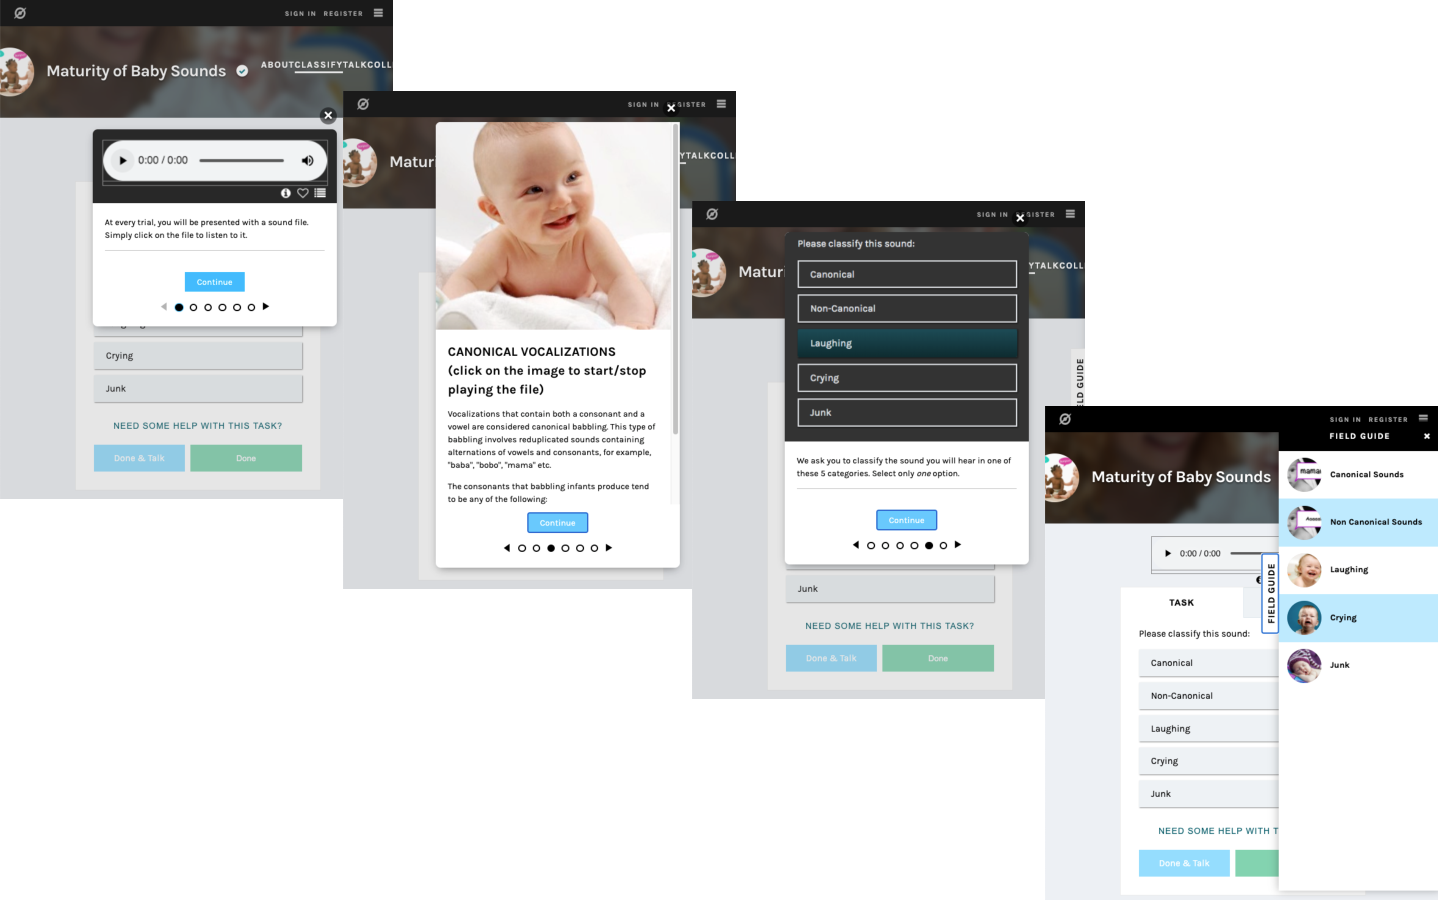
\includegraphics{zooniverse-pufig.pdf}
\caption{\label{fig:fig-zoo}Screen captures of the 6 stages of the tutorial, three of which are shown here: The initial explanation of the trial, examples of canonical vocalizations, and the classification choice the user needed to make; as well as the Field Guide, which remained accessible on the right of the screen throughout the session, and which allowed users to revise examples of the different categories.}
\end{figure}

\begin{figure}
\centering
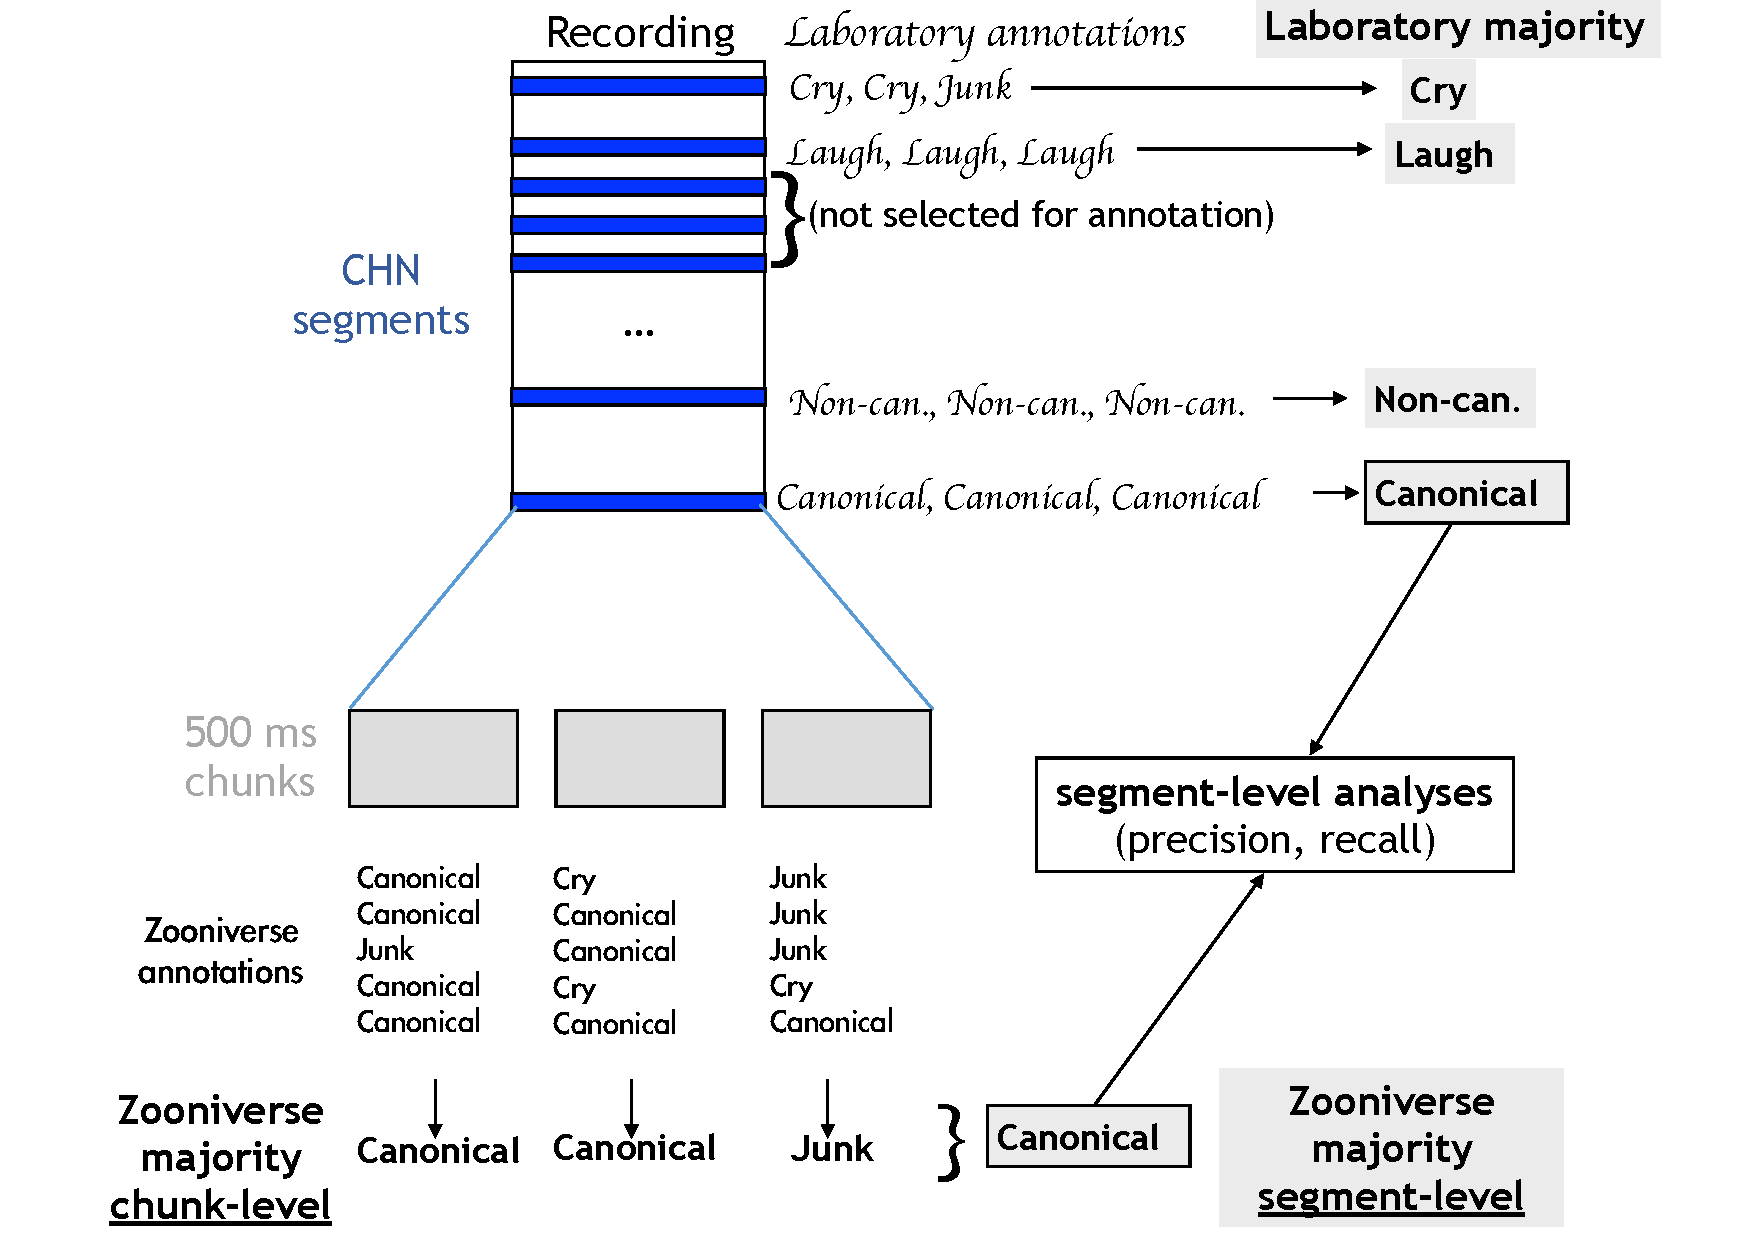
\includegraphics{fig_levels.key.pdf}
\caption{\label{fig:fig-process}Correspondence between LENA-identified segments (which can contain one or more vocalizations) and chunks. Segments and chunks are collectively referred to as clips because they are parts of the longer audio recording. Notice that clips are first annotated by multiple people, and these judgments are then combined into a single label based on simple majority. To compare laboratory and Zooniverse annotations at the level of segments, chunk-level labels are combined using the hierarchy Canonical \textgreater{} Non-canonical \textgreater{} Crying \textgreater{} Laughing \textgreater{} Junk.}
\end{figure}

\begin{figure}
\centering
\includegraphics{paper_files/figure-latex/fig-corage-1.pdf}
\caption{\label{fig:fig-corage}Correlations between child-level descriptors and age as a function of metric (Linguistic Proportion in the top row, Canonical Proportion in the bottom row), annotation method, and child group (red circles = low-risk, and black crosses = Angelman syndrome).}
\end{figure}

\begin{figure}
\centering
\includegraphics{paper_files/figure-latex/fig-prec-rec-1.pdf}
\caption{\label{fig:fig-prec-rec}Number of segments as a function of their majority label from laboratory annotations (rows) versus Zooniverse annotations (columns). Percentages (and shading) indicate precision (left) and recall (right). For precision, the percentage indicates what percentage of the segments that have a given majority label according to Zooniverse data are attributed a given label in Lab data (i.e., columns add up to 100\%). For recall, the percentage indicates what percentage of the segments that have a given majority label according to Lab data are attributed a given label in Zooniverse data (i.e., rows add up to 100\%).}
\end{figure}

\begin{figure}
\centering
\includegraphics{paper_files/figure-latex/fig-corlab-zoo-1.pdf}
\caption{\label{fig:fig-corlab-zoo}Correlations between child-level descriptors derived from Zooniverse data (y axis) versus lab data (x axis) as a function of child group (red circles = low-risk, and black crosses = Angelman syndrome).}
\end{figure}

\begin{figure}
\centering
\includegraphics{paper_files/figure-latex/fig-cor-Junk-1.pdf}
\caption{\label{fig:fig-cor-Junk}Correlations between child-level descriptors derived from Zooniverse data (y axis) versus lab data (x axis) as a function of whether children's Junk proportion was higher or lower than the median for all children (light blue wheels = lower, and green diamonds = higher).}
\end{figure}

\begin{table}

\caption{\label{tab:tab-LENA-challenge}Comparison of recall percentages obtained with the baseline algorithm created by the ComParE team, in the context of the ComParE 2019 BabySounds subchallenge (Schuller et al., 2019; C2019B), LENA labels (note LENA did not distinguish between Canonical and Non-canonical in this analysis), and those obtained in this study through Zooniverse annotations. Label frequency indicates the prevalence of the relevant label (Crying, Laughing, etc.) in each dataset (the same Lab dataset was used for both LENA and Zooniverse). UAR stands for unweighted average recall, WAR for weighted average recall (which takes into account label frequency).}
\centering
\begin{tabular}[t]{l|l|l|l|l|l}
\hline
 & C2019B & LENA & Zoon. & C2019B & Zoon.\\
\hline
Crying & 70.6 & 78.0 & 50.9 & 669 & 6762\\
\hline
Laughing & 41.5 & 56.0 & 62.9 & 149 & 409\\
\hline
Non-can. & 24.1 & 77.0 & 78.9 & 4485 & 1441\\
\hline
Canonical & 66.4 & 59.0 & 58.3 & 1426 & 1657\\
\hline
Junk & 67.3 & 1.0 & 43.5 & 4575 & 999\\
\hline
UAR & 54.0 & 41.0 & 58.9 &  & \\
\hline
WAR & 49.9 & 57.0 & 55.3 &  & \\
\hline
\end{tabular}
\end{table}

\begin{table}

\caption{\label{tab:tab-cors}Pearson correlation coefficients across metrics derived from laboratory and Zooniverse annotations in the Angelman syndrome (AS) group data, low-risk (LR) group data, or for all children together (all) in three ways. First, All seg indicates that Zooniverse annotations at the chunk level were first combined at the segment level. Second, Chunks indicates that they were analyzed directly at the chunk level. Both of these are based on all the data. Third, rows labeled 100 seg indicate that laboratory- and Zooniverse-derived metrics were based on only 100 segments (median over 50 runs in which 100 segments were randomly selected from each child).}
\centering
\begin{tabular}[t]{l|l|l}
\hline
  & Linguistic Proportion & Canonical Proportion\\
\hline
All seg AS & .89 & .855\\
\hline
Chunks AS & .845 & .866\\
\hline
100 seg AS & .791 & .632\\
\hline
All seg LR & .83 & .966\\
\hline
Chunks LR & .841 & .974\\
\hline
100 seg LR & .787 & .943\\
\hline
All seg all & .821 & .938\\
\hline
Chunks all & .845 & .963\\
\hline
100 seg all & .771 & .905\\
\hline
\end{tabular}
\end{table}

\begin{table}

\caption{\label{tab:tab-corage}Pearson correlation coefficients between derived metrics (Linguistic Proportion = LP; Canonical Proportion = CP) and age, for the Angelman syndrome (AS) group data and low-risk (LR) group data. Metrics were derived from laboratory annotations at the segment level (lab); from Zooniverse annotations collapsed at the segment level (Zoon. Seg); or directly from the chunk-level labels (Zoon. Chunks). }
\centering
\begin{tabular}[t]{l|l|l}
\hline
  & AS & LR\\
\hline
LP (lab) & .015 & .741\\
\hline
LP (Zoon. Seg.) & -.131 & .672\\
\hline
LP (Zoon. Chunks) & -.038 & .716\\
\hline
CP (lab) & -.557 & .607\\
\hline
CP (Zoon. Seg.) & -.404 & .604\\
\hline
CP (Zoon. Chunks) & -.38 & .573\\
\hline
\end{tabular}
\end{table}

\hypertarget{references}{%
\section{References}\label{references}}

\setlength{\parindent}{-0.5in}
\setlength{\leftskip}{0.5in}

\hypertarget{refs}{}
\leavevmode\hypertarget{ref-aust2017papaja}{}%
Aust, F., \& Barth, M. (2017). Papaja: Create APA manuscripts with R Markdown.

\leavevmode\hypertarget{ref-baumer2015r}{}%
Baumer, B., \& Udwin, D. (2015). R markdown. \emph{Wiley Interdisciplinary Reviews: Computational Statistics}, \emph{7}(3), 167--177.

\leavevmode\hypertarget{ref-belardi2017retrospective}{}%
Belardi, K., Watson, L. R., Faldowski, R. A., Hazlett, H., Crais, E., Baranek, G. T., \ldots{} Oller, D. K. (2017). A retrospective video analysis of canonical babbling and volubility in infants with Fragile X Syndrome at 9--12 months of age. \emph{Journal of Autism and Developmental Disorders}, \emph{47}(4), 1193--1206.

\leavevmode\hypertarget{ref-berinsky2012evaluating}{}%
Berinsky, A. J., Huber, G. A., \& Lenz, G. S. (2012). Evaluating online labor markets for experimental research: Amazon.com's Mechanical Turk. \emph{Political Analysis}, \emph{20}(3), 351--368.

\leavevmode\hypertarget{ref-borne2011zooniverse}{}%
Borne, K., \& Zooniverse Team. (2011). The zooniverse: A framework for knowledge discovery from citizen science data. \emph{AGUFM}, \emph{2011}, ED23C--0650.

\leavevmode\hypertarget{ref-bowyer2015panoptes}{}%
Bowyer, A., Lintott, C., Hines, G., Allan, C., \& Paget, E. (2015). Panoptes, a project building tool for citizen science. In \emph{Proceedings of the AAAI Conference on Human Computation and Crowdsourcing (HCOMP'15)}. San Diego, CA.

\leavevmode\hypertarget{ref-casillas2017new}{}%
Casillas, M., Bergelson, E., Warlaumont, A. S., Cristia, A., Soderstrom, M., VanDam, M., \& Sloetjes, H. (2017). A new workflow for semi-automatized annotations: Tests with long-form naturalistic recordings of children's language environments. In \emph{Interspeech 2017} (pp. 2098--2102).

\leavevmode\hypertarget{ref-casillas2019step}{}%
Casillas, M., \& Cristia, A. (2019). A step-by-step guide to collecting and analyzing long-format speech environment (LFSE) recordings. \emph{Collabra}, \emph{5}(1).

\leavevmode\hypertarget{ref-cristia2020accuracy}{}%
Cristia, A., Bulgarelli, F., \& Bergelson, E. (2020). Accuracy of the Language Environment Analysis system segmentation and metrics: A systematic review. \emph{Journal of Speech, Language, and Hearing Research}, \emph{63}(4), 1093--1105.

\leavevmode\hypertarget{ref-cristia2020thorough}{}%
Cristia, A., Lavechin, M., Scaff, C., Soderstrom, M., Rowland, C., Räsänen, O., \ldots{} Bergelson, E. (2020). A thorough evaluation of the Language Environment Analysis (LENA) system. \emph{Behavior Research Methods}, 1--20.

\leavevmode\hypertarget{ref-crump2013evaluating}{}%
Crump, M. J., McDonnell, J. V., \& Gureckis, T. M. (2013). Evaluating Amazon's Mechanical Turk as a tool for experimental behavioral research. \emph{PloS One}, \emph{8}(3), e57410.

\leavevmode\hypertarget{ref-cychosz2021canonical}{}%
Cychosz, M., Cristia, A., Bergelson, E., Casillas, M., Baudet, G., Warlaumont, A. S., \ldots{} Seidl, A. (2021). Canonical babble development in a large-scale crosslinguistic corpus.

\leavevmode\hypertarget{ref-Dykstra2013}{}%
Dykstra, J. R., Sabatos-Devito, M. G., Irvin, D. W., Boyd, B. A., Hume, K. A., \& Odom, S. L. (2013). Using the Language Environment Analysis (LENA) system in preschool classrooms with children with autism spectrum disorders. \emph{Autism}, \emph{17}(5), 582--594. \url{https://doi.org/https://doi.org/10.1177/1362361312446206}

\leavevmode\hypertarget{ref-Elo}{}%
Elo, H. (2016). \emph{Acquiring language as a twin}. Tampere, Finland: Tampere University Press.

\leavevmode\hypertarget{ref-fasolo2008babbling}{}%
Fasolo, M., Majorano, M., \& D'Odorico, L. (2008). Babbling and first words in children with slow expressive development. \emph{Clinical Linguistics \& Phonetics}, \emph{22}(2), 83--94.

\leavevmode\hypertarget{ref-ganek2018language}{}%
Ganek, H., \& Eriks-Brophy, A. (2018). Language ENvironment analysis (LENA) system investigation of day long recordings in children: A literature review. \emph{Journal of Communication Disorders}, \emph{72}, 77--85.

\leavevmode\hypertarget{ref-halpern2016excessive}{}%
Halpern, R., \& Coelho, R. (2016). Excessive crying in infants. \emph{Jornal de Pediatria}, \emph{92}(3), S40--S45.

\leavevmode\hypertarget{ref-hamrick2019capturing}{}%
Hamrick, L., Seidl, A., \& Kelleher, B. (2019). Capturing variability in early language skills among children with Angelman syndrome: A novel semi-automated approach. \emph{Presented at the Angelman Biomarkers and Outcome Measures Alliance Scientific Meeting}.

\leavevmode\hypertarget{ref-hamrick2019measurement}{}%
Hamrick, L., \& Tonnsen, B. (2019). Measurement and characterization of early social communication in children with Angelman syndrome. In A. Sadhwani \& K. Okoniewski (Eds.), \emph{Advances in characterizing developmental trajectories in Angelman syndrome across the lifespan, Gatlinburg conference}. San Antonio, TX.

\leavevmode\hypertarget{ref-heckman2006skill}{}%
Heckman, J. J. (2006). Skill formation and the economics of investing in disadvantaged children. \emph{Science}, \emph{312}(5782), 1900--1902.

\leavevmode\hypertarget{ref-kaya2020combining}{}%
Kaya, H., Verkholyak, O., Markitantov, M., \& Karpov, A. (2020). Combining clustering and functionals based acoustic feature representations for classification of baby sounds. In \emph{Companion publication of the 2020 international conference on multimodal interaction} (pp. 509--513).

\leavevmode\hypertarget{ref-lavechin2020open}{}%
Lavechin, M., Bousbib, R., Bredin, H., Dupoux, E., \& Cristia, A. (2020). An open-source voice type classifier for child-centered daylong recordings. \emph{Proceedings of Interspeech}. \url{https://doi.org/https://arxiv.org/abs/2005.12656v2}

\leavevmode\hypertarget{ref-mcdaniel2020predicting}{}%
McDaniel, J., Yoder, P., Estes, A., \& Rogers, S. J. (2020). Predicting expressive language from early vocalizations in young children with autism spectrum disorder: Which vocal measure is best? \emph{Journal of Speech, Language, and Hearing Research}, \emph{63}(5), 1509--1520.

\leavevmode\hypertarget{ref-oller2000emergence}{}%
Oller, D. (2000). The emergence of the capacity for speech. Mahwah, NJ: Erlbaum.

\leavevmode\hypertarget{ref-oller1998late}{}%
Oller, D. K., Eilers, R. E., Neal, A. R., \& Cobo-Lewis, A. B. (1998). Late onset canonical babbling: A possible early marker of abnormal development. \emph{American Journal on Mental Retardation}, \emph{103}(3), 249--263.

\leavevmode\hypertarget{ref-oller2010automated}{}%
Oller, D. K., Niyogi, P., Gray, S., Richards, J. A., Gilkerson, J., Xu, D., \ldots{} Warren, S. F. (2010). Automated vocal analysis of naturalistic recordings from children with autism, language delay, and typical development. \emph{Proceedings of the National Academy of Sciences}, \emph{107}(30), 13354--13359.

\leavevmode\hypertarget{ref-overby2020retrospective}{}%
Overby, M., Belardi, K., \& Schreiber, J. (2020). A retrospective video analysis of canonical babbling and volubility in infants later diagnosed with childhood apraxia of speech. \emph{Clinical Linguistics \& Phonetics}, \emph{34}(7), 634--651.

\leavevmode\hypertarget{ref-rankine2017language}{}%
Rankine, J., Li, E., Lurie, S., Rieger, H., Fourie, E., Siper, P. M., \ldots{} Kolevzon, A. (2017). Language ENvironment Analysis (LENA) in Phelan-McDermid syndrome: Validity and suggestions for use in minimally verbal children with Autism Spectrum Disorder. \emph{Journal of Autism and Developmental Disorders}, \emph{47}(6), 1605--1617.

\leavevmode\hypertarget{ref-team2013r}{}%
R Core Team, \& others. (2013). R: A language and environment for statistical computing.

\leavevmode\hypertarget{ref-roche2018early}{}%
Roche, L., Zhang, D., Bartl-Pokorny, K. D., Pokorny, F. B., Schuller, B. W., Esposito, G., \ldots{} others. (2018). Early vocal development in autism spectrum disorder, Rett syndrome, and Fragile X syndrome: Insights from studies using retrospective video analysis. \emph{Advances in Neurodevelopmental Disorders}, \emph{2}(1), 49--61.

\leavevmode\hypertarget{ref-schuller2019interspeech}{}%
Schuller, B. W., Batliner, A., Bergler, C., Pokorny, F. B., Krajewski, J., Cychosz, M., \ldots{} others. (2019). The INTERSPEECH 2019 Computational Paralinguistics Challenge: Styrian Dialects, Continuous Sleepiness, Baby Sounds \& Orca Activity. In \emph{Interspeech} (pp. 2378--2382).

\leavevmode\hypertarget{ref-Seidl19}{}%
Seidl, A., Warlaumont, A., \& Cristia, A. (2019). Towards detection of canonical babbling by citizen scientists: Performance as a function of clip length. In \emph{Interspeech} (pp. 3579--3583). \url{https://doi.org/10.21437/Interspeech.2019-1773}

\leavevmode\hypertarget{ref-semenzin2020zooniverse}{}%
Semenzin, C., \& Cristia, A. (2020). Zooniverse pipeline for long format recordings. Retrieved from \url{https://github.com/LAAC-LSCP/Zooniverse}

\leavevmode\hypertarget{ref-sescleifer2018systematic}{}%
Sescleifer, A. M., Francoisse, C. A., \& Lin, A. Y. (2018). Systematic review: Online crowdsourcing to assess perceptual speech outcomes. \emph{Journal of Surgical Research}, \emph{232}, 351--364.

\leavevmode\hypertarget{ref-vandam2016homebank}{}%
Vandam, M., Warlaumont, A. S., Bergelson, E., Cristia, A., Soderstrom, M., De Palma, P., \& Macwhinney, B. (2016). HomeBank: An online repository of daylong child-centered audio recordings. \emph{Seminars in Speech and Language}, \emph{37}(2), 128--142. \url{https://doi.org/10.1055/s-0036-1580745}

\leavevmode\hypertarget{ref-vandam2019use}{}%
VanDam, M., \& Yoshinaga-Itano, C. (2019). Use of the LENA Autism Screen with children who are deaf or hard of hearing. \emph{Medicina}, \emph{55}(8), 495.

\leavevmode\hypertarget{ref-wang2020meta}{}%
Wang, Y., Williams, R., Dilley, L., \& Houston, D. M. (2020). A meta-analysis of the predictability of LENA™ automated measures for child language development. \emph{Developmental Review}, \emph{57}, 100921.

\leavevmode\hypertarget{ref-xu2008signal}{}%
Xu, D., Yapanel, U., Gray, S., Gilkerson, J., Richards, J., \& Hansen, J. (2008). Signal processing for young child speech language development. In \emph{First Workshop on Child, Computer and Interaction}.

\leavevmode\hypertarget{ref-yao2020classification}{}%
Yao, X., Micheletti, M., Johnson, M., \& Barbaro, K. de. (2020). Classification of infant crying in real-world home environments using deep learning. \emph{arXiv Preprint arXiv:2005.07036}.

\leavevmode\hypertarget{ref-yeh2019using}{}%
Yeh, S.-L., Chao, G.-Y., Su, B.-H., Huang, Y.-L., Lin, M.-H., Tsai, Y.-C., \ldots{} others. (2019). Using attention networks and adversarial augmentation for Styrian dialect, continuous sleepiness and baby sound recognition. In \emph{INTERSPEECH} (pp. 2398--2402).

\clearpage
\renewcommand{\listfigurename}{Figure captions}


\end{document}
